\documentclass[8pt]{beamer}

\newif\ifplacelogo % create a new conditional
\placelogotrue % set it to true

\usetheme{Warsaw}
\usecolortheme{rose}
\usepackage{multicol}
\usepackage{epstopdf}
\usepackage[italic]{hepnames}
\usepackage{tikz}
\usepackage{listings}
\usepackage{times}
\usepackage{amsmath}
\usepackage{verbatim}
\usepackage{hyperref}
\usepackage{bbding}
\lstset{breakatwhitespace,
language=C++,
columns=fullflexible,
keepspaces,
breaklines,
tabsize=3, 
showstringspaces=false,
extendedchars=true}

% TikZ includes!!!
\usepackage{tikz}
\usetikzlibrary{backgrounds}
\usetikzlibrary{calc}
\tikzstyle{every picture}+=[remember picture]
\input{/home/oviazlo/Desktop/beamerPresentations/myReports/latexHelpScripts/tikzGrid.tex}


\begin{document}

% custom colors
\definecolor{olive}{rgb}{0.3, 0.4, .1}
\definecolor{fore}{RGB}{249,242,215}
\definecolor{back}{RGB}{51,51,51}
\definecolor{title}{RGB}{255,0,90}
\definecolor{dgreen}{rgb}{0.,0.6,0.}
\definecolor{gold}{rgb}{1.,0.84,0.}
\definecolor{JungleGreen}{cmyk}{0.99,0,0.52,0}
\definecolor{BlueGreen}{cmyk}{0.85,0,0.33,0}
\definecolor{RawSienna}{cmyk}{0,0.72,1,0.45}
\definecolor{Magenta}{cmyk}{0,1,0,0}

\definecolor{PixelColor}{RGB}{207,232,139}
\definecolor{SCTColor}{RGB}{167,166,255}
\definecolor{TRTColor}{RGB}{250,224,140}
\definecolor{grayColor}{RGB}{153,153,153}

\newcommand{\yRefPosOne}{0.0}
\newcommand{\xRefPosOne}{0.0}
\newcommand{\yRefPosTwo}{0.0}
\newcommand{\xRefPosTwo}{0.0}
\newcommand{\yRefIncrementOne}{0.0}
\newcommand{\xRefIncrementOne}{0.0}
\newcommand{\yRefIncrementTwo}{0.0}
\newcommand{\xRefIncrementTwo}{0.0}

\graphicspath{ {/home/oviazlo/Desktop/beamerPresentations/FCCee/pictures/} }
\DeclareGraphicsExtensions{.eps, .pdf, .png}

\newcommand{\myBox}[2][pink] {
    \noindent\colorbox{#1}{
	\textbf{#2}
    }\par
}

% For nice block (provided by Oleh)
\tikzstyle{mybox} = [draw=red, fill=blue!1, very thick,
    rectangle, rounded corners, inner sep=5pt, inner ysep=9pt]
    
\tikzstyle{PixelBox} = [draw=PixelColor, fill=blue!1, very thick,
    rectangle, rounded corners, inner sep=5pt, inner ysep=9pt]
\tikzstyle{SCTBox} = [draw=SCTColor, fill=blue!1, very thick,
    rectangle, rounded corners, inner sep=5pt, inner ysep=9pt]
\tikzstyle{TRTBox} = [draw=TRTColor, fill=blue!1, very thick,
    rectangle, rounded corners, inner sep=5pt, inner ysep=9pt]

% poster advertisement
\newcommand{\myCenterBox}[2][pink] {
   {\centering
    \noindent\colorbox{#1}{
	\textbf{#2}
    }\par
  }
}

\newcommand{\mySmallCenterBox}[2][pink] {
   {\centering
    \noindent\colorbox{#1}{
	\textbf{{\small #2}}
    }\par
  }
}

\newcommand{\myVerySmallCenterBox}[2][pink] {
   {\centering
    \noindent\colorbox{#1}{
	\textbf{{\scriptsize #2}}
    }\par
  }
}

\newcommand{\backupbegin}{
   \newcounter{finalframe}
   \setcounter{finalframe}{\value{framenumber}}
}
\newcommand{\backupend}{
   \setcounter{framenumber}{\value{finalframe}}
}

\newcommand{\myNode}{\tikz[baseline,inner sep=1pt] \node[anchor=base]}

\definecolor{light-gray}{gray}{0.95}
% poster advertisement


\title[ CLIC-inspired detector for FCC-ee \hspace{13.5em}\insertframenumber/
\inserttotalframenumber]{ Tracking and single particle performance with the CLIC-inspired detector for FCC-ee }


	\author[Oleksandr Viazlo, Emilia Leogrande]{Oleksandr Viazlo, Emilia Leogrande \\ 
% 	{\small ???}
	}
	\institute{\small CERN\\} 
	
       
	\date{10 October 2017}

% 	\logo{ \ifplacelogo \includegraphics[height=1.8cm]{./ID_week2/lund_uni-logo_s.pdf} \hspace{0.4cm} \fi}

	
   	\frame{\titlepage}

   	

\placelogofalse

%*****************************************************************************
\begin{frame}{\large \large Introduction}
 
 \begin{itemize}
  \item ???
 \end{itemize}

 
\end{frame}
%*****************************************************************************



%*****************************************************************************
\begin{frame}{\large \large FCC-ee detector model}
 
\renewcommand{\yRefPosOne}{0}
\renewcommand{\xRefPosOne}{5.3}
\renewcommand{\xRefIncrementOne}{5.5}
\begin{tikzpicture}[overlay]

\node [Box] at (\xRefPosOne,\yRefPosOne) (box){%
    \begin{minipage}{0.99\textwidth}
      \begin{itemize}
	\item Update on detector model (FCCee$\_$o5$\_$v04). Implementation of carbon support structures in the VTX and Tracker.
      \end{itemize}
    \end{minipage}
};


%  \node[TRTBox] (tmp) at (\xRefPosOne-3,\yRefPosOne-2.5)
%   { 
%     \begin{minipage}{0.5\textwidth}
% 
%     \resizebox{\columnwidth}{!}{%
%       \begin{tabular}{lccc}
% 	 & CLIC & & FCC-ee \\[0.18cm]
% 	VTX Barrel & 31-60 mm & $\Longrightarrow$ & 17-59 mm \\[0.18cm]
% 	VTX Endcap & Spirals & $\Longrightarrow$ & Disks \\[0.18cm]
% 	Tracker Radius & 1486 mm & $\Longrightarrow$ & 2100 mm \\[0.18cm]
%       \end{tabular}%
%     }
%     \end{minipage}
%   };
%   
%  \node[TRTBox] (tmp) at (\xRefPosOne+3.2,\yRefPosOne-2.5)
%   { 
%     \begin{minipage}{0.54\textwidth}
% 
%     \resizebox{\columnwidth}{!}{%
%       \begin{tabular}{lccc}
% 	 & CLIC & & FCC-ee \\[0.18cm]
% 	ECAL thickness & 202 mm & $\Longrightarrow$ & 202 mm \\[0.18cm]
% 	HCAL thickness & 44 $\times$ 7.5 $\lambda_0$ & $\Longrightarrow$ & 44 $\times$ 5.5 $\lambda_0$ \\[0.18cm]
% 	Yoke Thickness & 1989 mm & $\Longrightarrow$ & 1521 mm \\[0.18cm]
%       \end{tabular}%
%     }
%     \end{minipage}
%   };
% 
% \node [Box] at (\xRefPosOne,\yRefPosOne-1) (box){%
% \myCenterBox{Overall dimensions of CLIC and FCC-ee detectors}
% };
  
\end{tikzpicture}
\end{frame}
%*****************************************************************************




%*****************************************************************************
\begin{frame}{\large \large Summary and outlook}
 
 
 
 
 \renewcommand{\yRefPosOne}{0}
\renewcommand{\xRefPosOne}{5.3}
\renewcommand{\xRefIncrementOne}{5.5}
\begin{tikzpicture}[overlay]

      
\node [Box] at (\xRefPosOne,\yRefPosOne+2) (box){%
  \begin{minipage}{0.99\textwidth}
 \begin{itemize}
  \item Complete FCC-ee detector model is available for performance studies
  \item Tracking performance was studied with full simulation and reconstruction (truth tracking)
    \end{itemize}
  \end{minipage}
};
% \node[fancytitle, right=15pt] at (box.north west) {Transition Radiation Tracker};


\node [PixelBox] at (\xRefPosOne,\yRefPosOne-2) (box){%
  \begin{minipage}{0.99\textwidth}
 \begin{itemize}
     \item Conformal tracking performance (single $\mu$ and Z $\to$ uds events) \\[0.3cm]

     \item Effect of increased material budget in VTX \\[0.3cm]
     
     \item Calorimeter studies: 
     \begin{itemize}
      \item complex events - PID efficiency
      \item jet energy resolution
     \end{itemize}
     
     \item Overlay of beam background \\[0.3cm]

%      electron and photon PID efficiencies using the Pandora Particle Flow Algorithm, jets performance
    \end{itemize}
  \end{minipage}
};

\node [Box] at (\xRefPosOne-4.2,\yRefPosOne+0.4) (box){%
\myCenterBox[PixelColor]{Next steps}
};

% \node[fancytitle, right=15pt] at (box.north west) {Next steps};
% \node[fancytitle, right=15pt] at (box.north west) {LUCID};

\end{tikzpicture}
  
\end{frame}
%*****************************************************************************

%------------------------------------------------
\begin{frame}
\frametitle{BACKUP} 
 
\end{frame}
%------------------------------------------------

%*****************************************************************************
\begin{frame}{\large \large CLIC detector}

\renewcommand{\yRefPosOne}{0}
\renewcommand{\xRefPosOne}{5.3}
\renewcommand{\xRefIncrementOne}{5.5}
\begin{tikzpicture}[overlay]

 \node[inner sep=0pt] (tmp) at (\xRefPosOne-2.5,\yRefPosOne-0.5)
    {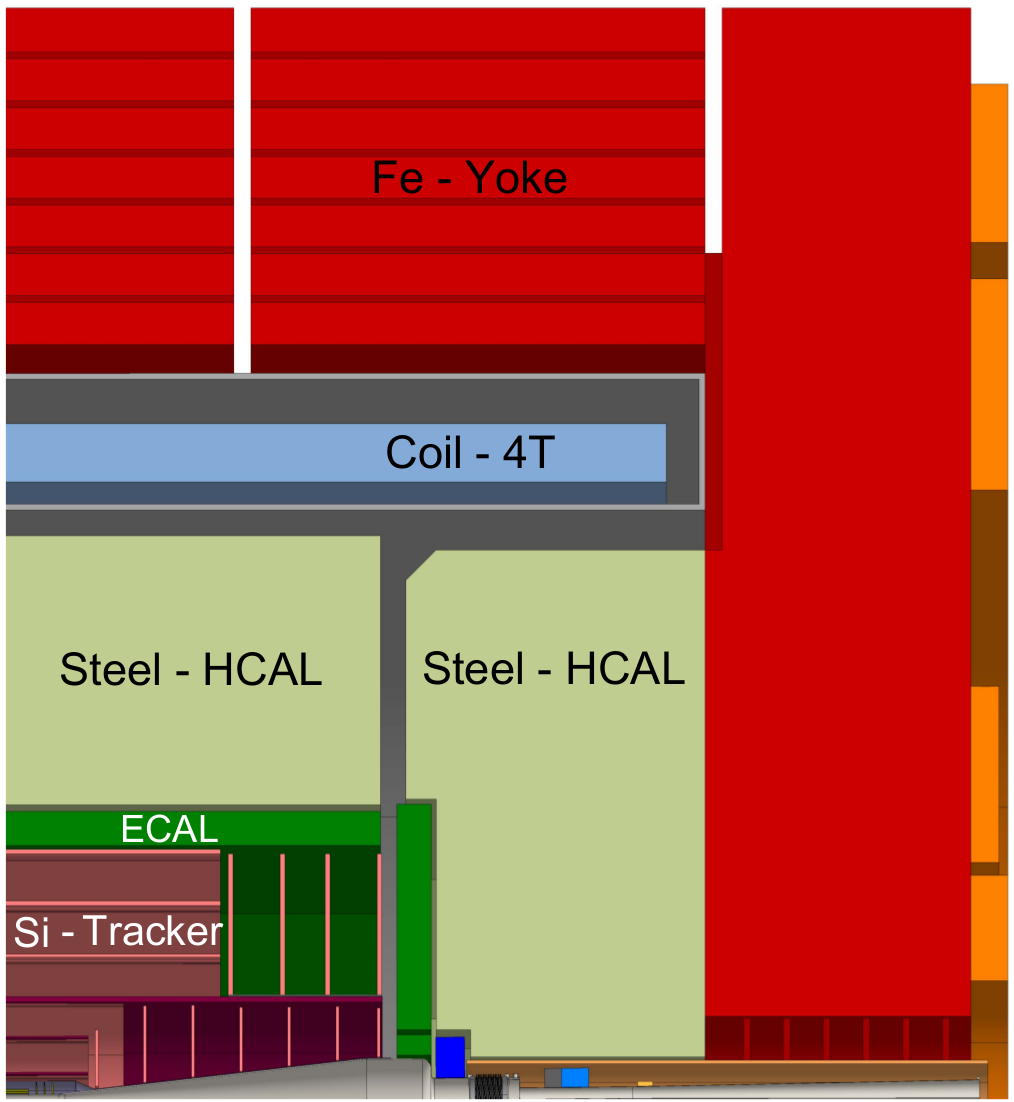
\includegraphics[width=7cm]{CLICdet.png}};

    
\node [Box] at (\xRefPosOne+3.5,\yRefPosOne+1.3) (box){%
    \begin{minipage}{0.5\textwidth}

  \begin{itemize}
   \item Full silicon VTX and Tracker: \\ $\geqslant$12 hits per track
   \item W-Si ECAL and Fe-Scint HCAL
   \item Coil is outside of the calorimeter; \\4 Tesla magnetic field
   \item Steel return yoke with 6 RPC muon chambers
  \end{itemize}

    \end{minipage}
};
% \node[fancytitle, right=15pt] at (box.north west) {Subdetectors};
\node [Box] at (\xRefPosOne+3.5,\yRefPosOne+3.2) (box){%
\myCenterBox{Subdetectors}
};


\node [Box] at (\xRefPosOne+3.5,\yRefPosOne-3) (box){%
    \begin{minipage}{0.5\textwidth}

  \begin{itemize}
   \item Momentum resolution (at 500 GeV): $\sigma_{\mathrm{p_T}}/ \mathrm{p_T}^2 \simeq 2\cdot10^{-5}$ GeV$^{-1}$
   \item Lepton ID efficiency: $>$ 95$\%$
   \item Impact parameter resolution: \\
	 $\sigma_{d_0} = a \oplus \dfrac{b}{p~sin^{3/2} \theta}$ \\ $a \leqslant $5$ \mu$m, $b \leqslant $15 $\mu$m GeV
   \item Jet energy resolution: \\
	 $\sigma_E / E \simeq $ 3.5 $\%$
 \end{itemize}

    \end{minipage}
};

\node [Box] at (\xRefPosOne+3.5,\yRefPosOne-0.9) (box){%
\myCenterBox{Detector requirements}
};


\node [Box] at (\xRefPosOne-0.15,\yRefPosOne+2.9) (box){%
\myCenterBox{CLIC}
};

% \node[fancytitle, right=15pt] at (box.north west) {Detector requirements};

%% HELPER draw advanced helping grid with axises:
% \draw(-0.5,-4) to[grid with coordinates] (11.5,4);
\end{tikzpicture}

 
\end{frame}
%*****************************************************************************

%*****************************************************************************
\begin{frame}{\large \large FCC-ee detector}
 
\renewcommand{\yRefPosOne}{0}
\renewcommand{\xRefPosOne}{5.3}
\renewcommand{\xRefIncrementOne}{5.5}
\begin{tikzpicture}[overlay]


 \node[TRTBox] (tmp) at (\xRefPosOne,\yRefPosOne-0.5)
  { 
    \begin{minipage}{0.8\textwidth}

    \resizebox{\columnwidth}{!}{%
      \begin{tabular}{lccc}
	 & CLIC & & FCC-ee \\[0.18cm]
	VTX Barrel & 31-60 mm & $\Longrightarrow$ & 17-59 mm \\[0.18cm]
	VTX Endcap & Spirals & $\Longrightarrow$ & Disks \\[0.18cm]
	Tracker radius & 1486 mm & $\Longrightarrow$ & 2100 mm \\[0.18cm]
% 	ECAL thickness & 202 mm & $\Longrightarrow$ & 202 mm \\[0.18cm]
% 	HCAL thickness & 44 $\times$ 7.5 $\lambda_0$ & $\Longrightarrow$ & 44 $\times$ 5.5 $\lambda_0$ \\[0.18cm]
	ECAL thickness & 40 layers, 22 X$_0$ & $\Longrightarrow$ & 40 layers, 22 X$_0$ \\[0.18cm]
	HCAL thickness & 60 layers, 7.5 $\lambda_I$ & $\Longrightarrow$ & 44 layers, 5.5 $\lambda_I$ \\[0.18cm]
	Yoke thickness & 1989 mm & $\Longrightarrow$ & 1521 mm \\[0.18cm]
	MDI (forward region) &  & $\Longrightarrow$ & $<$ 150 mrad \\[0.4cm]
	Solenoid field & 4 Tesla & $\Longrightarrow$ & 2 Tesla \\
	
      \end{tabular}%
    }
    \end{minipage}
  };
  


\node [Box] at (\xRefPosOne,\yRefPosOne+2.6) (box){%
\myCenterBox[TRTColor]{Overall dimensions of CLIC and FCC-ee detectors}
};
  
\end{tikzpicture}
\end{frame}
%*****************************************************************************


%*****************************************************************************
\begin{frame}{\large \large Tracking}

\renewcommand{\yRefPosOne}{0}
\renewcommand{\xRefPosOne}{5.3}
\renewcommand{\xRefIncrementOne}{5.5}
\begin{tikzpicture}[overlay]

 \node[inner sep=0pt] (tmp) at (\xRefPosOne,\yRefPosOne-1.4)
    {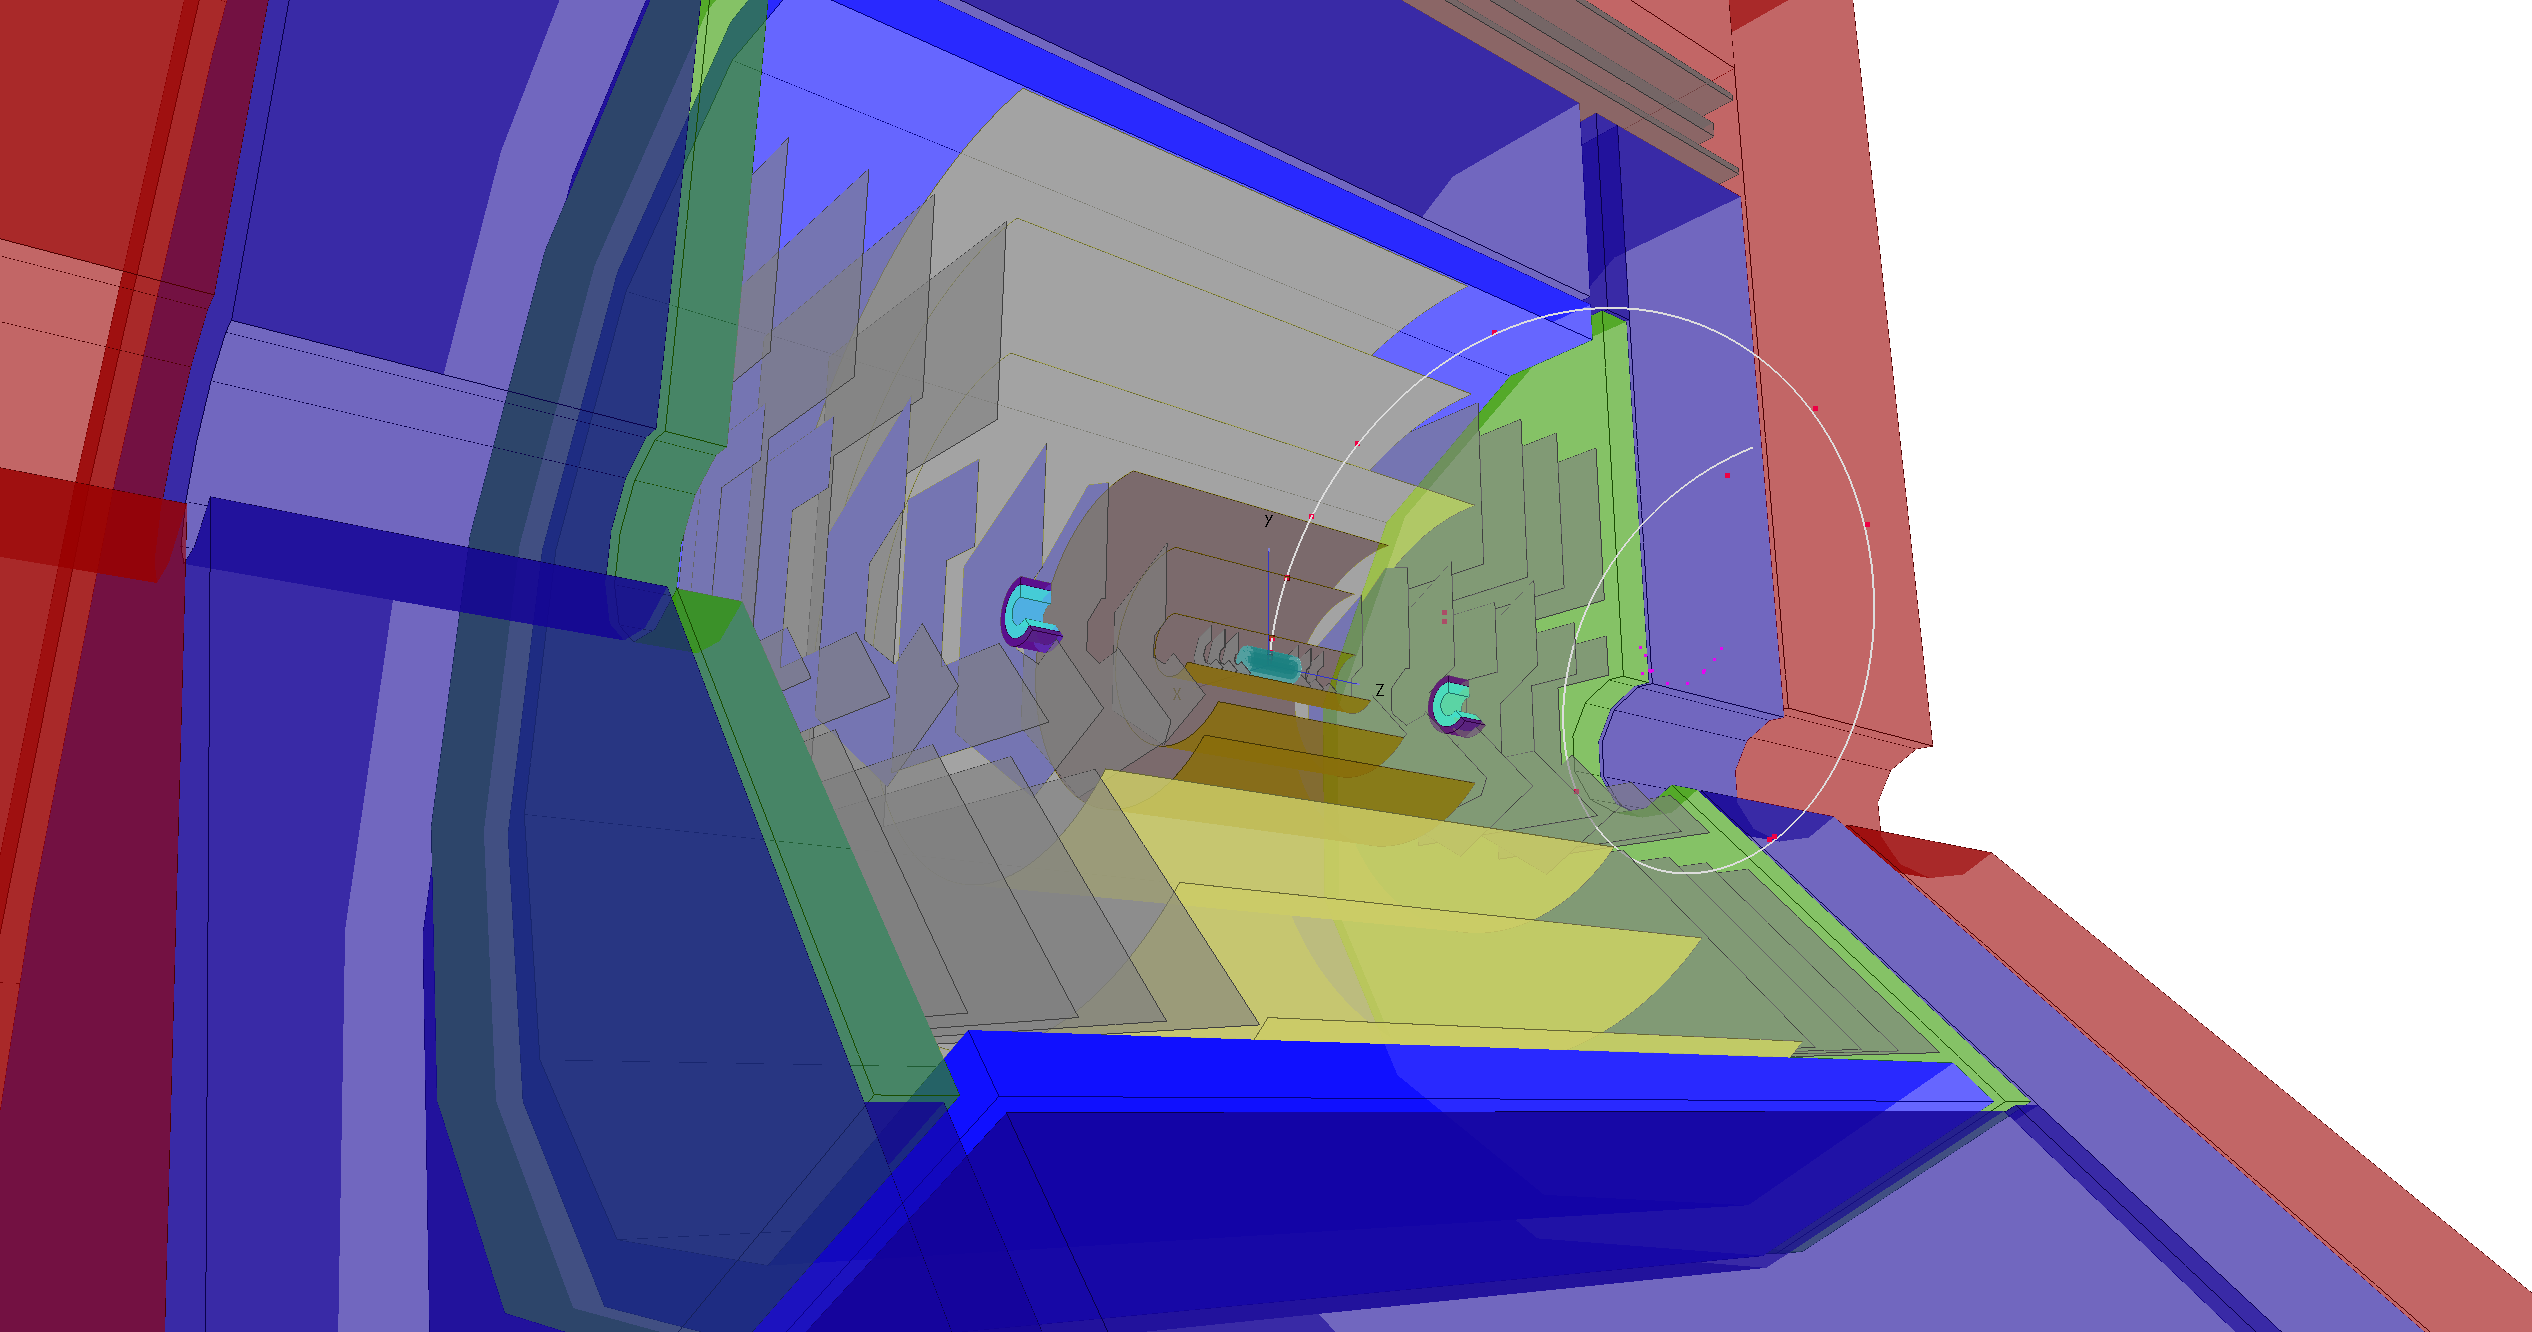
\includegraphics[width=10cm]{eventDisplay/eventDisplay_v1.png}};

    
\node [Box] at (\xRefPosOne,\yRefPosOne+2.57) (box){%
    \begin{minipage}{0.99\textwidth}

  \begin{itemize}
  \item Two tracking algorithms are available: 
  \begin{itemize}
   \item truth tracking - track fitting is done by using all hits produced by particle (by using truth information)
   \item conformal tracking - hits are found by pattern recognition algorithm in conformal space
  \end{itemize}
  \item Single-point resolution (sigma): VTX - 3$\times$3 $\mu$m; IT - 7$\times$300$\mu$m; OT - 7$\times$3000$\mu$m
 \end{itemize}

    \end{minipage}
};

\node [Box] at (\xRefPosOne,\yRefPosOne-4.4) (box){%
    \begin{minipage}{0.99\textwidth}

  \begin{itemize}
  \item Charged particles with p$_\mathrm{T} >$ 0.65 GeV reach calorimeter.
 \end{itemize}

    \end{minipage}
};

% \node[fancytitle, right=15pt] at (box.north west) {Transition Radiation Tracker};

\node [Box] at (\xRefPosOne+3.8,\yRefPosOne+0.5) (box){%
\myCenterBox{FCC-ee}
};


%% HELPER draw advanced helping grid with axises:
% \draw(-0.5,-4) to[grid with coordinates] (11.5,4);
\end{tikzpicture}

 
 


 
\end{frame}
%*****************************************************************************

\end{document}

